\documentclass[11pt]{article}
\usepackage[margin=1in]{geometry}
\usepackage{graphicx,booktabs,siunitx,float,caption,subcaption,amssymb}
\usepackage[section]{placeins}
\usepackage[hidelinks]{hyperref}
\captionsetup{font=small,labelfont=bf}
\sisetup{detect-all}
\graphicspath{{fig/}}
\setlength{\parskip}{4pt}
\setlength{\parindent}{0pt}

\title{FMCW Radar --- Simulation Results\\\large Horn antenna (HFSS) and baseband electronics (Multisim)}
\author{David Brown}
\date{October 2026}

\begin{document}
\maketitle

\section*{Summary}

This document records the simulations run to check that the radar's horn antenna and baseband
circuits work before they are built. The horn was simulated in Ansys HFSS (Student 2025 R2) and the
baseband cards in NI Multisim 14. The projects, exported data and plots are in the repository under
\texttt{hfss/} and \texttt{multisim/}.

\begin{itemize}
  \item \textbf{Horn:} with the feed probe moved to 27\,mm long and 17.7\,mm from the back wall,
        the horn is matched to better than $-24$\,dB across 2400--2483.5\,MHz, gives 13.1--13.3\,dBi
        gain, and couples $-49$\,dB into the receive horn. The original probe position
        (28\,mm / 43.7\,mm) only reached $-5$\,dB, so the build guide was updated.
  \item \textbf{Baseband:} every card passes. Card 8 (all blocks on one sheet) first failed. The cause
        was two op-amp supply pins left unconnected on the sheet, and fixing them exposed a real gain loss.
        C6 was raised from 47\,\si{\micro\farad} to 3.3\,mF to fix that (Section~\ref{sec:card8}).
\end{itemize}

%==========================================================================================
\section{Horn antenna}

\FloatBarrier
\subsection{Model}
The horn is an optimum-gain pyramidal horn on a WR-340 waveguide (Figure~\ref{fig:section}).
It is fed by an SMA connector on the top wall whose centre pin is extended into the guide as a
brass probe. The HFSS model uses perfect-conductor walls, a 50\,\si{\ohm} coax wave port, and a
radiation boundary 40\,mm from the horn. Gain and beamwidth are fixed by the flare; the only things
that need tuning are the probe length and its distance from the back wall.

\begin{figure}[htbp]
  \centering
  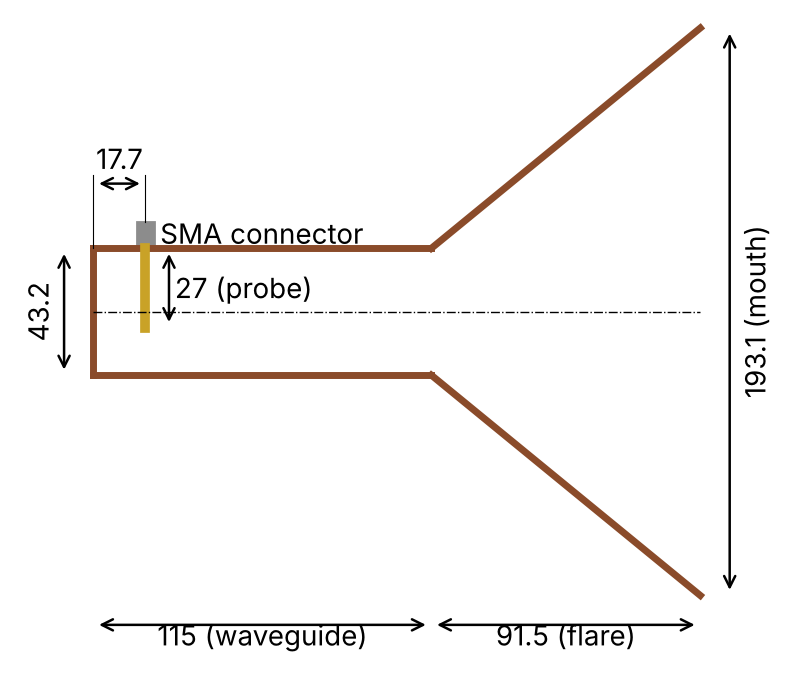
\includegraphics[width=0.62\linewidth]{horn_section}
  \caption{Side section of the horn (inside dimensions in mm) with the final probe position:
  27\,mm long, centre 17.7\,mm from the back wall. The mouth is 263.8\,mm wide in the other plane.}
  \label{fig:section}
\end{figure}

\FloatBarrier
\subsection{Why the first design did not match}
The original design placed the probe a quarter guide-wavelength (43.7\,mm) from the back wall, the
usual textbook rule. In simulation that gave $|S_{11}| = -5.2$\,dB at best: about 30\% of the power
reflected. De-embedding the simulated $S_{11}$ to the base of the probe shows it sees about
$95 - j76$\,\si{\ohm}, roughly twice the resistance needed and capacitive. Changing the probe length
alone cannot fix both. Moving the back wall closer lowers the resistance and adds inductance that
cancels the capacitance; at 17.7\,mm the probe sees $52 + j3$\,\si{\ohm} (Figure~\ref{fig:diag}).

\begin{figure}[htbp]
  \centering
  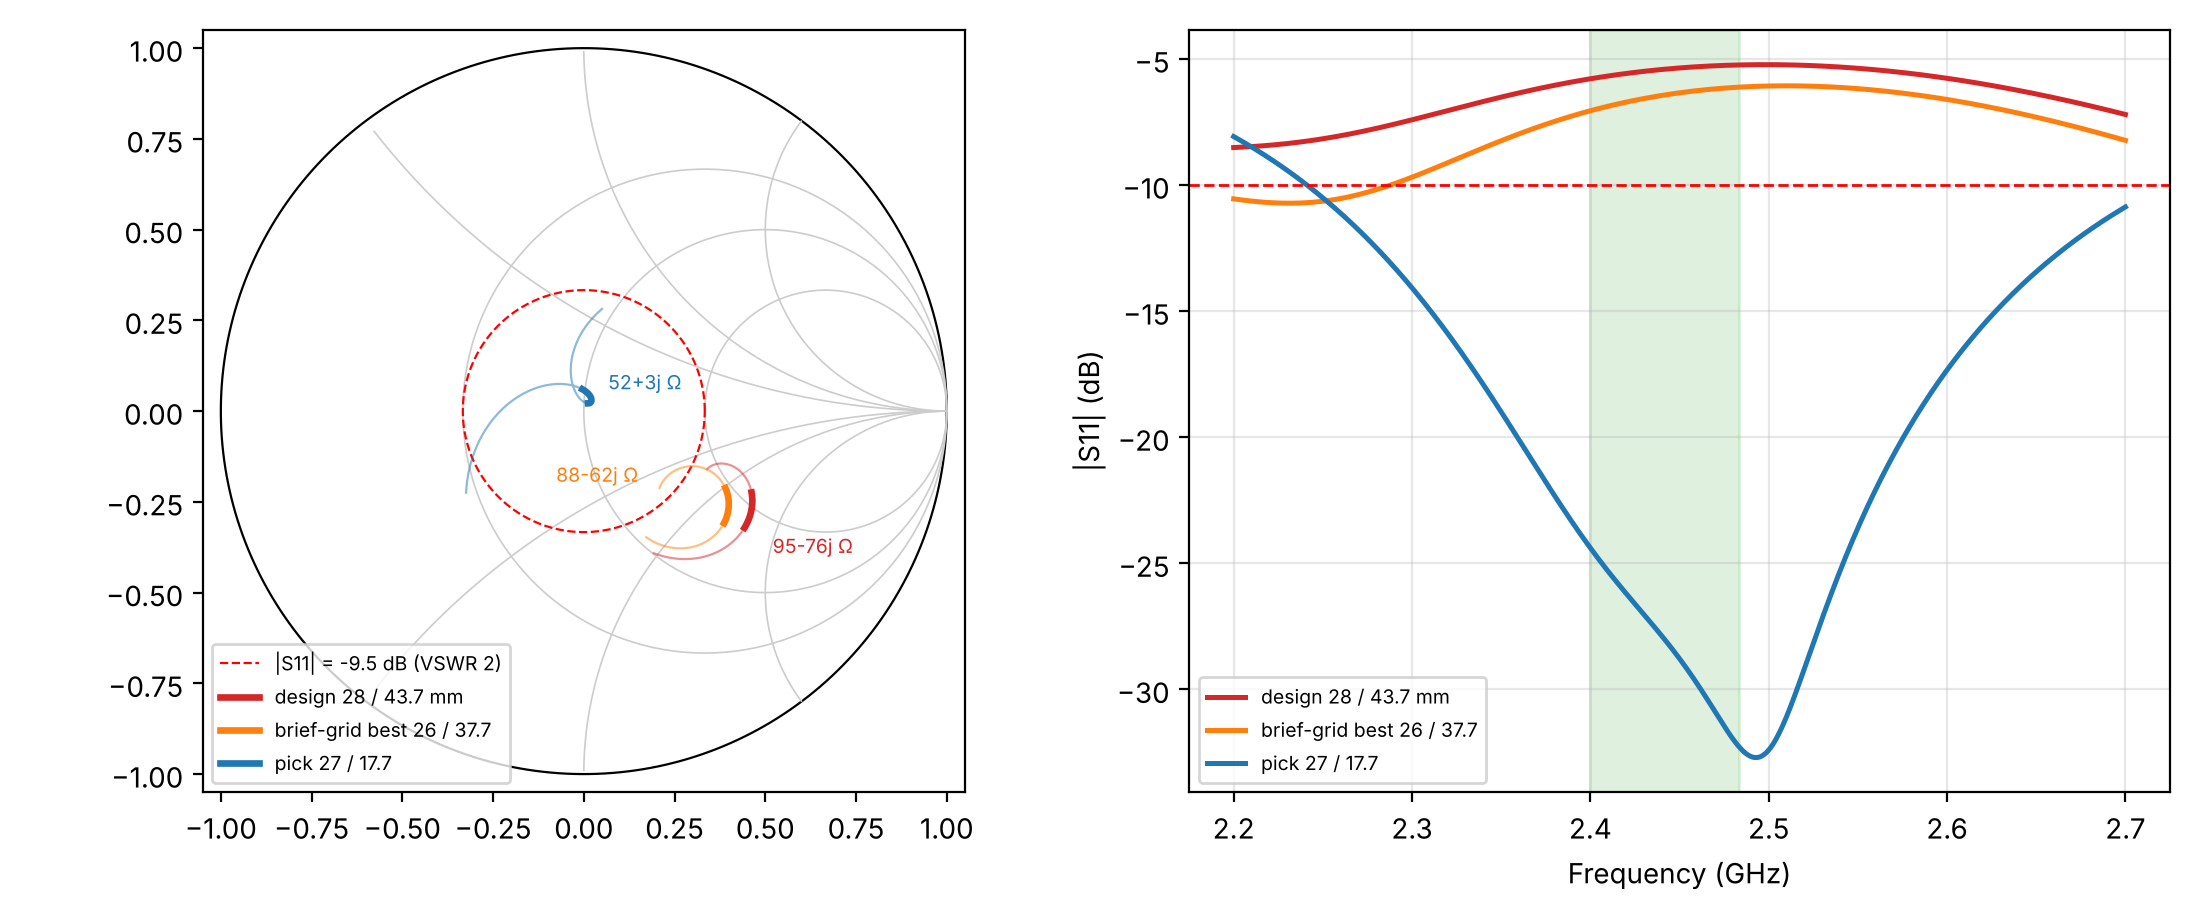
\includegraphics[width=\linewidth]{scan_diagnosis}
  \caption{Left: impedance at the probe base on a Smith chart for the original design (red),
  the best point on the original sweep grid (orange) and the final position (blue); the dashed
  circle is $-9.5$\,dB. Right: the matching $|S_{11}|$ curves.}
  \label{fig:diag}
\end{figure}

\FloatBarrier
\subsection{Choosing the probe position}
A 1\,mm grid of 57 solves (probe length 25--29\,mm, back-wall distance 12.7--22.7\,mm) was run. Since
a hand-built horn will not land exactly on the drawing, each point was scored by the worst
$S_{11}$ anywhere within $\pm1$\,mm of it. The best point is 27\,mm / 17.7\,mm: $-24.4$\,dB itself
and no worse than $-14.5$\,dB anywhere in the $\pm1$\,mm box (Figure~\ref{fig:scan}). Probe length is
the more sensitive dimension (1\,mm too long costs about 9\,dB), so it should be cut long and trimmed.

\begin{figure}[htbp]
  \centering
  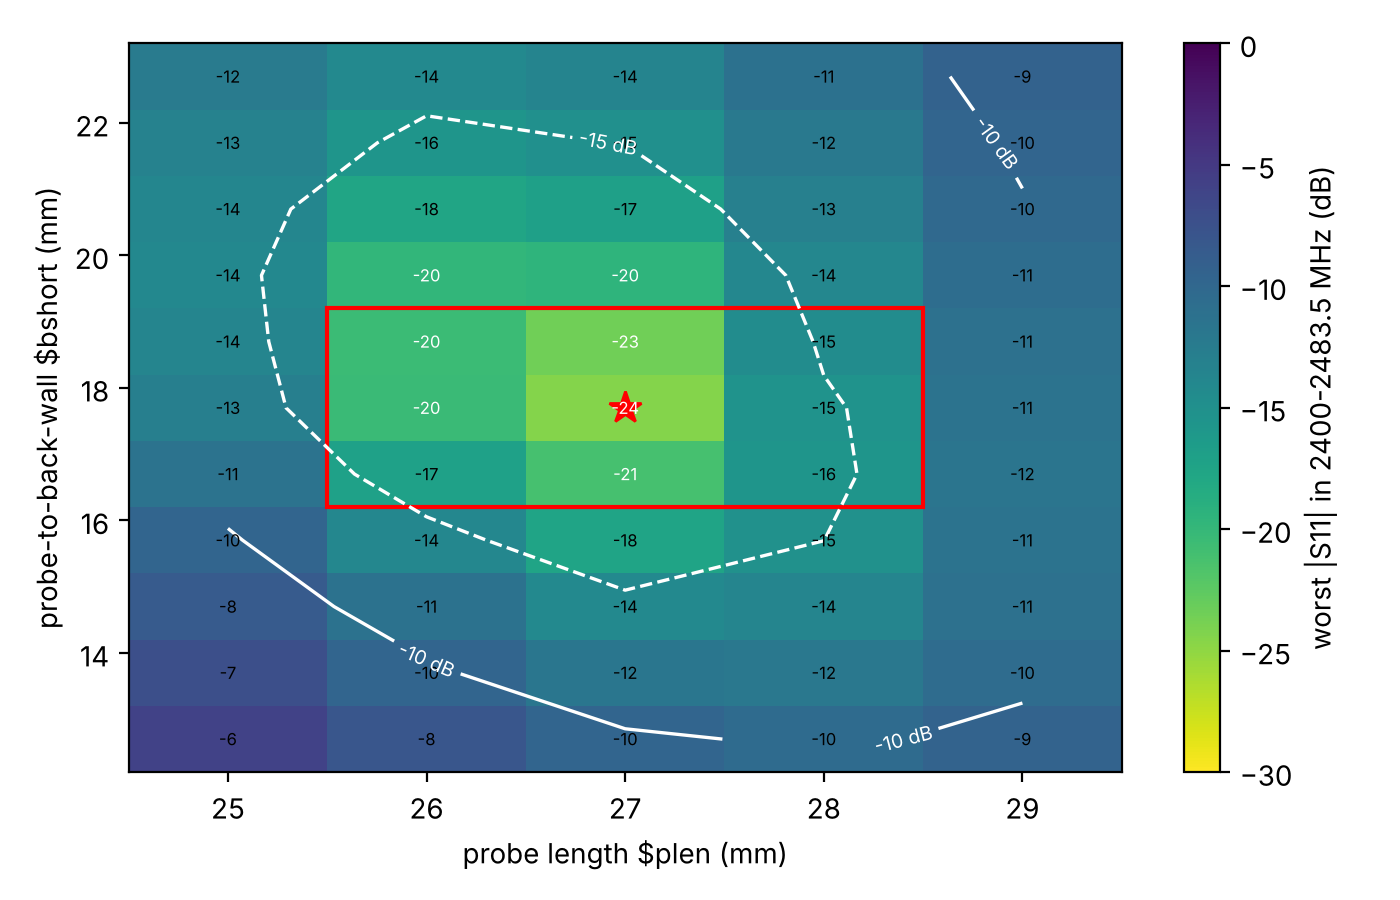
\includegraphics[width=0.65\linewidth]{scan_heatmap}
  \caption{Worst $|S_{11}|$ in 2400--2483.5\,MHz for every point of the 1\,mm scan. The red box is the
  $\pm1$\,mm build tolerance around the chosen point (star).}
  \label{fig:scan}
\end{figure}

\FloatBarrier
\subsection{Results at the final probe position}
\begin{table}[H]
  \centering
  \begin{tabular}{lll}
    \toprule
    Quantity & Simulated & Requirement \\
    \midrule
    Worst $|S_{11}|$, 2400--2483.5\,MHz & $-24.3$\,dB & $\le -10$\,dB \\
    Realized gain (2.400 / 2.442 / 2.4835\,GHz) & 13.24 / 13.24 / 13.27\,dBi & 12.5--14\,dBi \\
    E-plane / H-plane half-power beamwidth & 34.4\si{\degree} / 36.4\si{\degree} & theory 33.4\si{\degree} / 35.2\si{\degree} \\
    TX $\to$ RX coupling, horns 290\,mm apart & $-49.4$\,dB & $\le -35$\,dB \\
    Convergence & $\Delta S = 0.0026$, 7 passes & $\le 0.01$ \\
    \bottomrule
  \end{tabular}
  \caption{Final solve (11{,}909 tetrahedra). Every requirement is met.}
  \label{tab:horn}
\end{table}

\begin{figure}[htbp]
  \centering
  \begin{subfigure}{0.49\linewidth}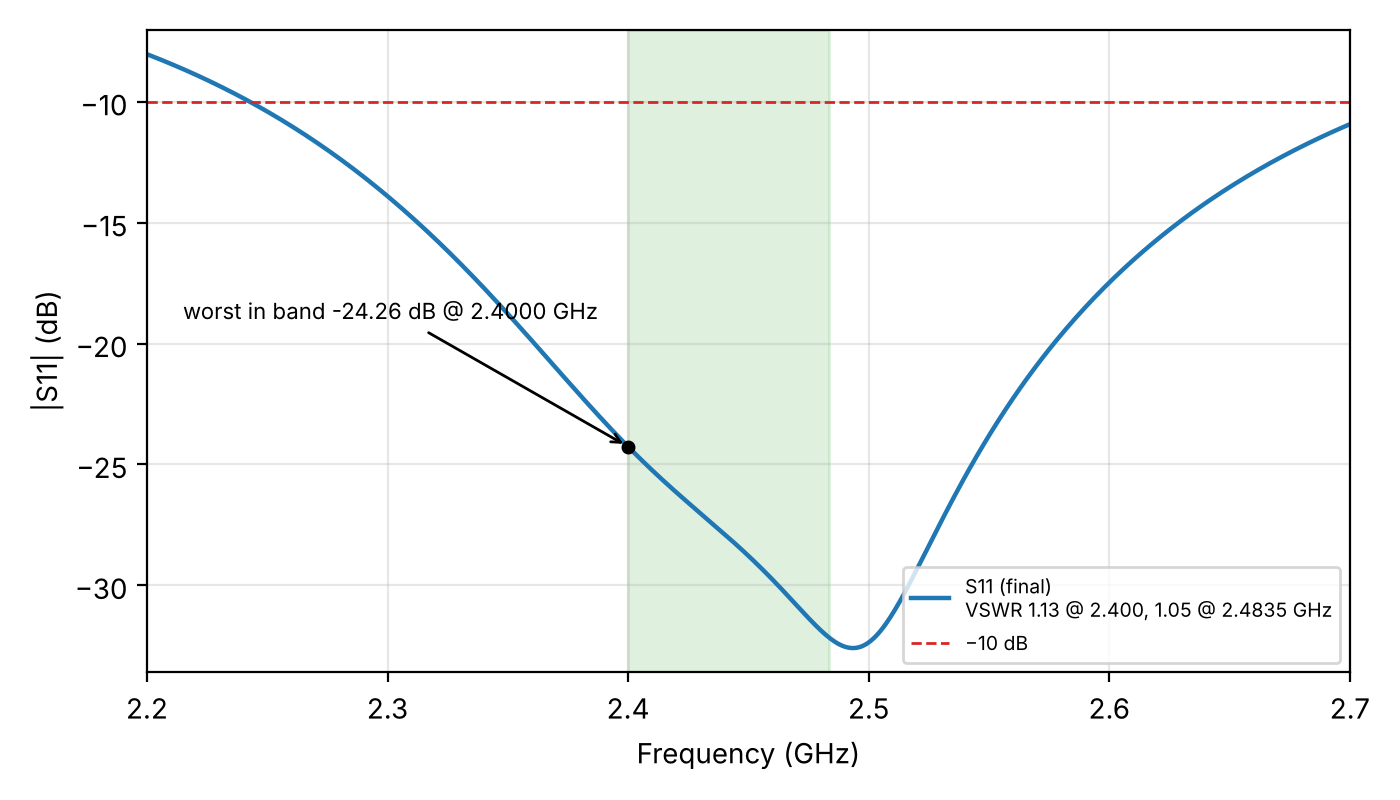
\includegraphics[width=\linewidth]{s11}\caption{$|S_{11}|$}\end{subfigure}
  \begin{subfigure}{0.49\linewidth}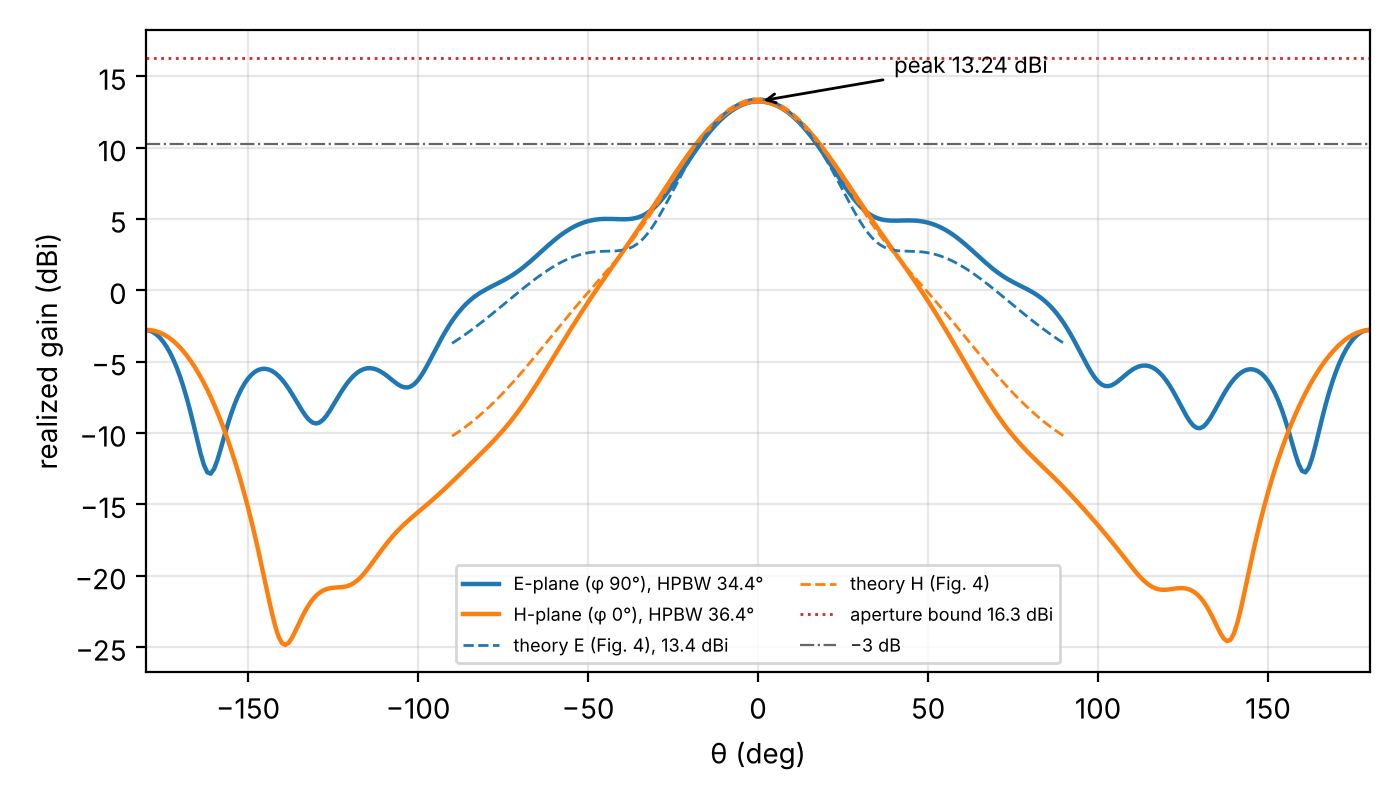
\includegraphics[width=\linewidth]{patterns}\caption{Gain cuts at 2.45\,GHz}\end{subfigure}
  \caption{(a) Input match; the shaded band is 2400--2483.5\,MHz. (b) Realized gain in the E- and
  H-planes against the aperture-integration theory (dashed).}
  \label{fig:final}
\end{figure}

\begin{figure}[htbp]
  \centering
  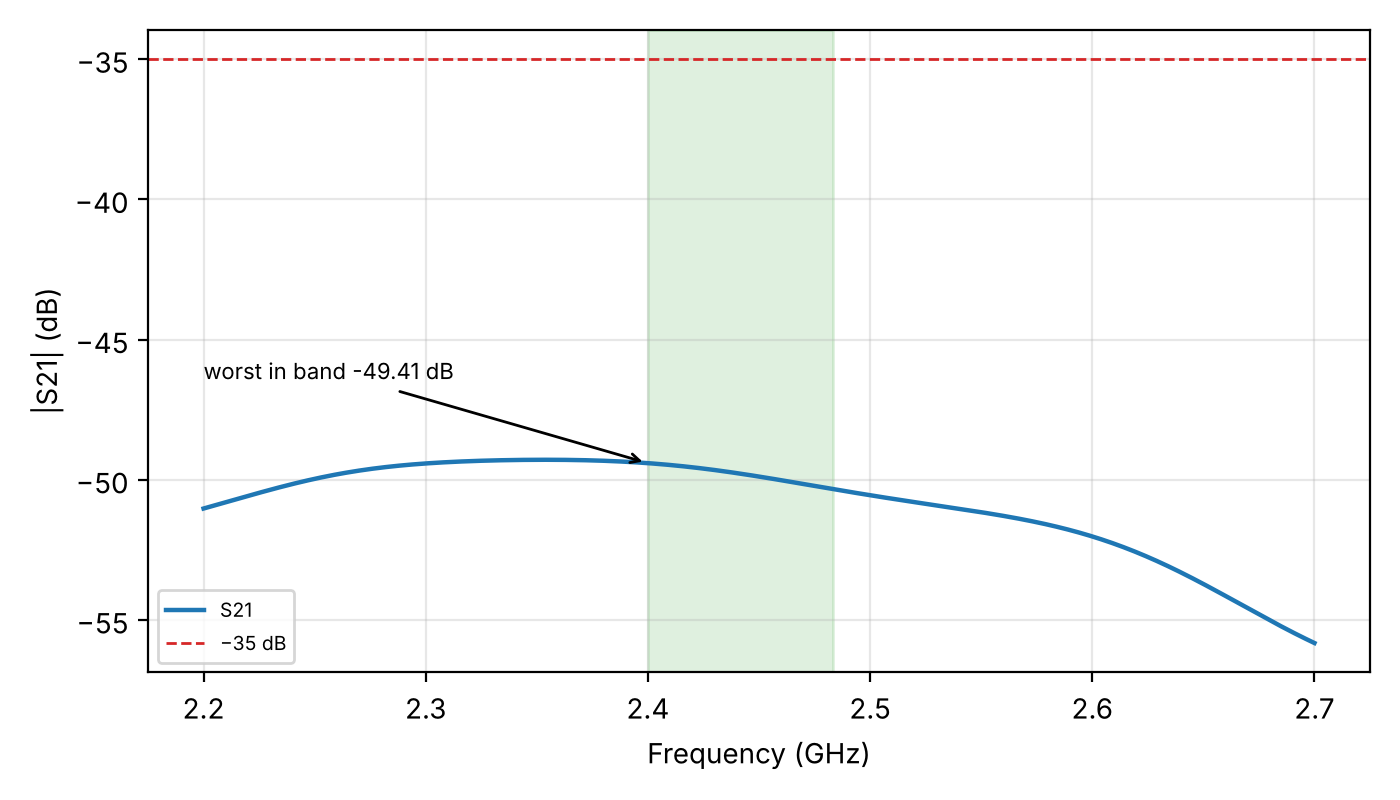
\includegraphics[width=0.6\linewidth]{isolation}
  \caption{Coupling from the transmit horn into the receive horn, side by side 290\,mm apart.}
  \label{fig:iso}
\end{figure}

\FloatBarrier
\subsection{Is the result trustworthy?}
Two checks were run at the final probe position:
\begin{itemize}
  \item \textbf{Mesh:} the same horn was solved on a coarse (8{,}773), the final (11{,}909) and a fine
        (28{,}825 tetrahedra) mesh. Gain changed by 0.14\,dB and $S_{11}$ stayed between $-22$ and
        $-24$\,dB (Figure~\ref{fig:mesh}), so the answer does not depend on the mesh. (The Student
        licence refuses meshes above roughly 67{,}000 elements.)
  \item \textbf{Copper:} replacing the perfect-conductor walls and probe with copper changed the gain
        by $+0.01$\,dB and $S_{11}$ from $-24.3$ to $-24.1$\,dB. Conductor loss is negligible.
\end{itemize}

\begin{figure}[htbp]
  \centering
  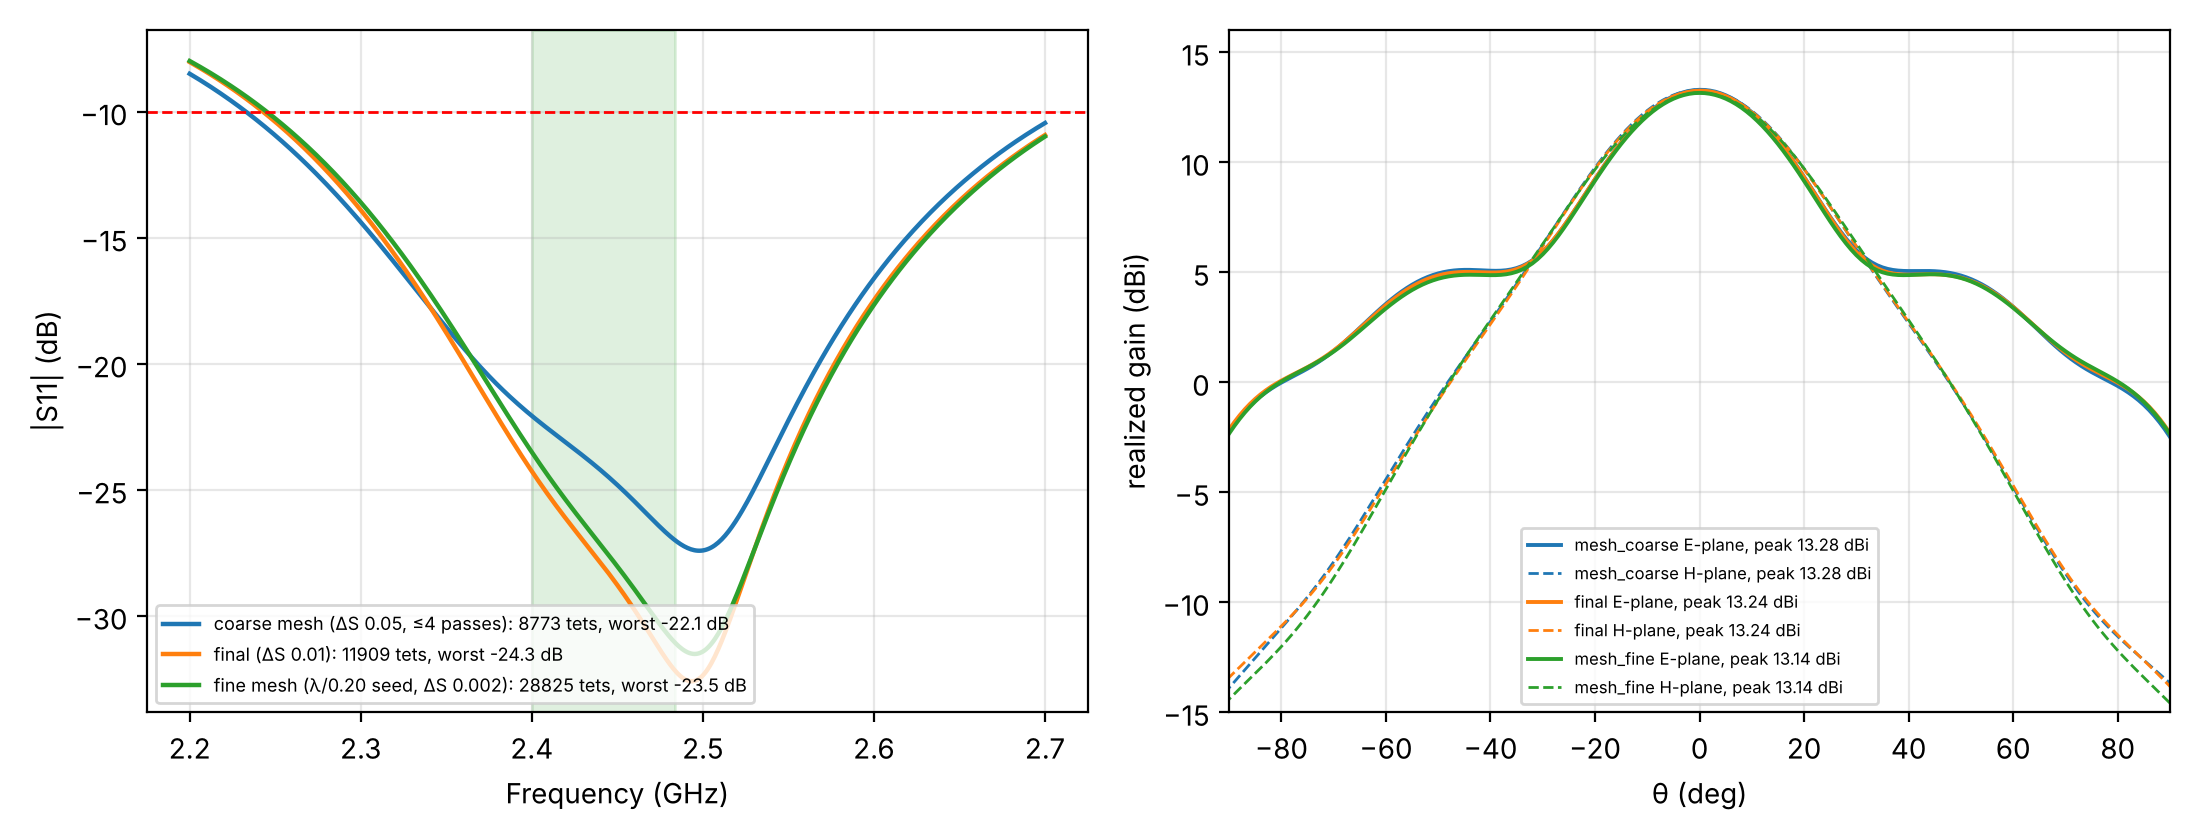
\includegraphics[width=\linewidth]{robust_mesh}
  \caption{$|S_{11}|$ (left) and gain cuts (right) on three meshes.}
  \label{fig:mesh}
\end{figure}

Not modelled: solder seams, the SMA connector's internal transition, and the bench surroundings.
Seams should be soldered continuously; if the measured match is off, trim the probe in 0.5\,mm steps.

%==========================================================================================
\clearpage
\section{Baseband electronics (Multisim)}

Each card is one block of the baseband board, simulated with library parts and checked against
its expected values. Results are in \texttt{multisim/}.

\begin{table}[htbp]
  \centering
  \footnotesize
  \setlength{\tabcolsep}{4pt}
  \begin{tabular}{lllc}
    \toprule
    Card & Check & Simulated (expected) & \\
    \midrule
    1 Video amp & DC: outputs -- vref & 1.07\,mV ($\le150$\,mV) & \checkmark \\
                & Gain at 159\,Hz / 1\,kHz / 15.9\,kHz & 48.7 / 54.5 / 50.9\,dB (48.7 / 54.5 / 50.6) & \checkmark \\
                & 1\,kHz output, 0.5\,mVpk in & 0.266\,Vpk (0.27) & \checkmark \\
                & First power-up peak & 106.8\,mVpk (107) & \checkmark \\
                & Clipping & $\pm4.06$\,V (about $\pm4.2$) & \checkmark \\
                & Two-tone: 417 / 870\,Hz lines & 19.1 / 21.1\,mVpk (19.0 / 21.2) & \checkmark \\
    2 Half-rail ref & vdiv / vref & 5.70 / 5.58\,V (5.70 / 5.58--5.72) & \checkmark \\
                & 150\,kHz rejection to vref & $-162$\,dB ($\le -100$) & \checkmark \\
    3 Power entry & vprot / vana & 11.72 / 11.62\,V (11.68 / 11.58) & \checkmark \\
                & Ripple on vana & 3.2\,mVpp (about 4) & \checkmark \\
                & Filter $-3$\,dB corner & 159\,Hz (a few hundred Hz) & \checkmark \\
    4 Reverse supply & vprot with $-12$\,V in & $-11$\,mV ($|v| < 0.5$\,V) & \checkmark \\
    5 Sync divider & High / low level & 275 / 1.4\,mV (270--300 / 0) & \checkmark \\
    6 IF input & ap at 417 / 870\,Hz & $-6.64$ / $-6.19$\,dB ($-6.6$ / $-6.2$) & \checkmark \\
                & if at 2.44\,GHz & $-57.7$\,dB ($-57.7$) & \checkmark \\
    7 Radar (scaled) & Beat at 5 / 10 / 15\,m & 435.0 / 870.7 / 1305.8\,Hz (435.2 / 870.4 / 1305.6) & \checkmark \\
    8 Full board & DC: outputs -- vref & 1.1\,mV ($\le 150$\,mV) & \checkmark \\
                & Gain vs.\ card 1, 10\,Hz--50\,kHz & within 0.15\,dB ($\le 0.3$) & \checkmark \\
                & Two-tone 870\,Hz line / 150\,kHz ripple & 21.0\,mVpk / 0.06\,\si{\micro\volt}pp (21.2 / $<1$\,mV) & \checkmark \\
                & Power-up, outputs settle at vref & 0.53\,s, no latch-up ($<1$\,s) & \checkmark \\
    \bottomrule
  \end{tabular}
  \caption{Multisim checks. Card 8 is the corrected sheet (Section~\ref{sec:card8}).}
  \label{tab:ms}
\end{table}

\FloatBarrier
\subsection{Card 1: video amplifier}
The three-stage TL072 amplifier matches the hand-calculated response at all three test frequencies
(Figure~\ref{fig:amp}a). With an 870\,Hz beat tone 46\,dB below a large 12.5\,Hz interferer, both lines
come through at the expected levels (Figure~\ref{fig:amp}b), so the high-pass stages do their job.

\begin{figure}[htbp]
  \centering
  \begin{subfigure}{0.49\linewidth}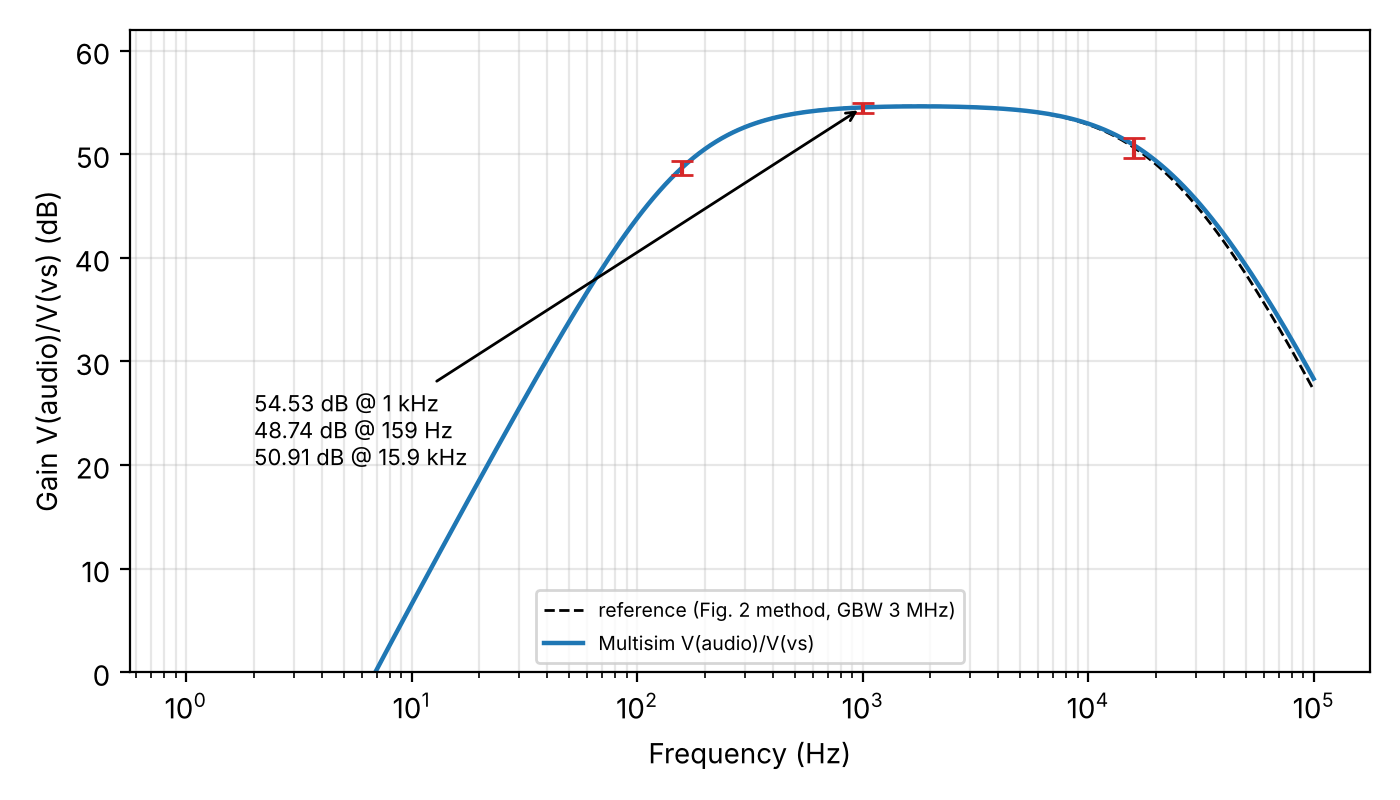
\includegraphics[width=\linewidth]{01_bode}\caption{Gain vs.\ frequency}\end{subfigure}
  \begin{subfigure}{0.49\linewidth}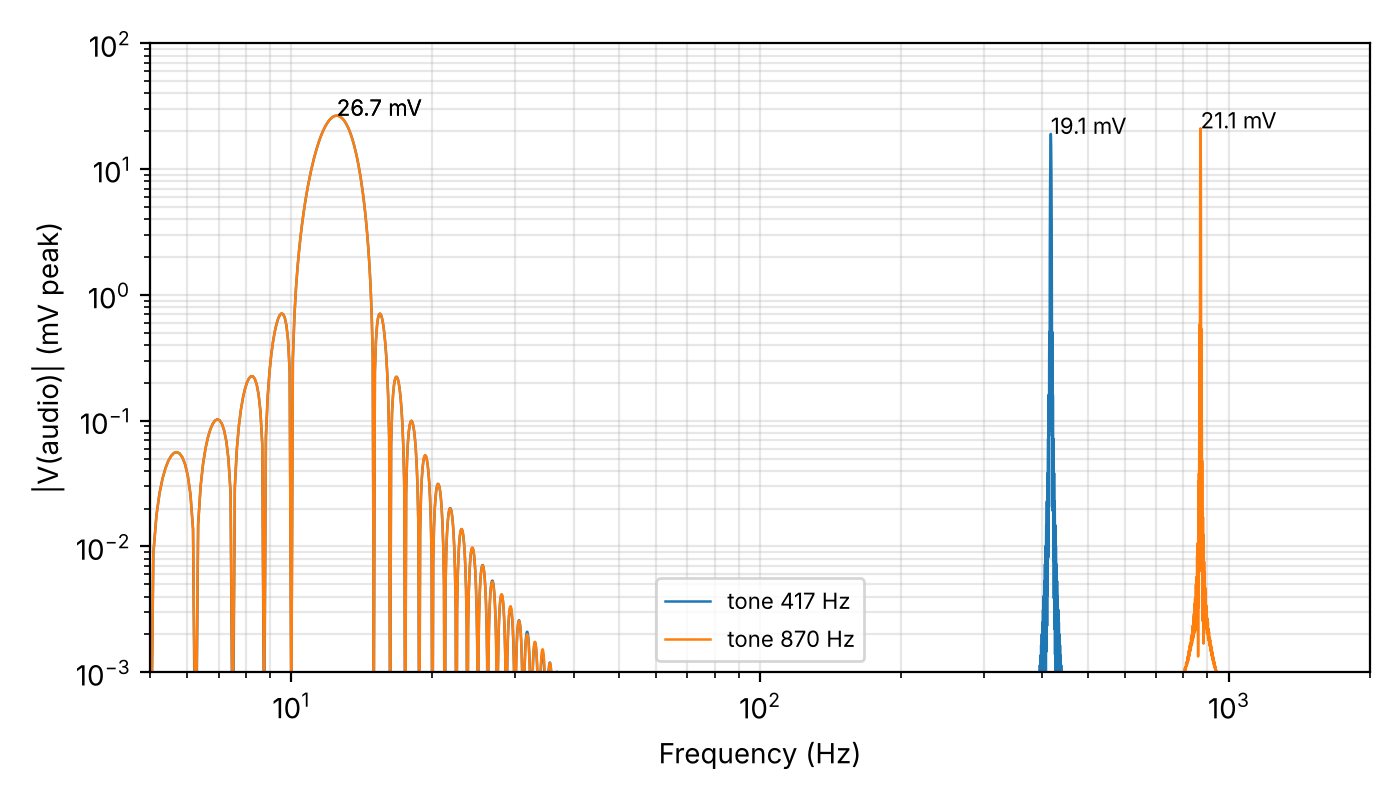
\includegraphics[width=\linewidth]{01d_twotone_spectrum}\caption{Two-tone spectrum}\end{subfigure}
  \caption{Card 1. (a) Simulated gain against the reference curve; red bars are the pass bands.
  (b) Output spectrum for 12.5\,Hz + 417/870\,Hz input.}
  \label{fig:amp}
\end{figure}

\begin{figure}[htbp]
  \centering
  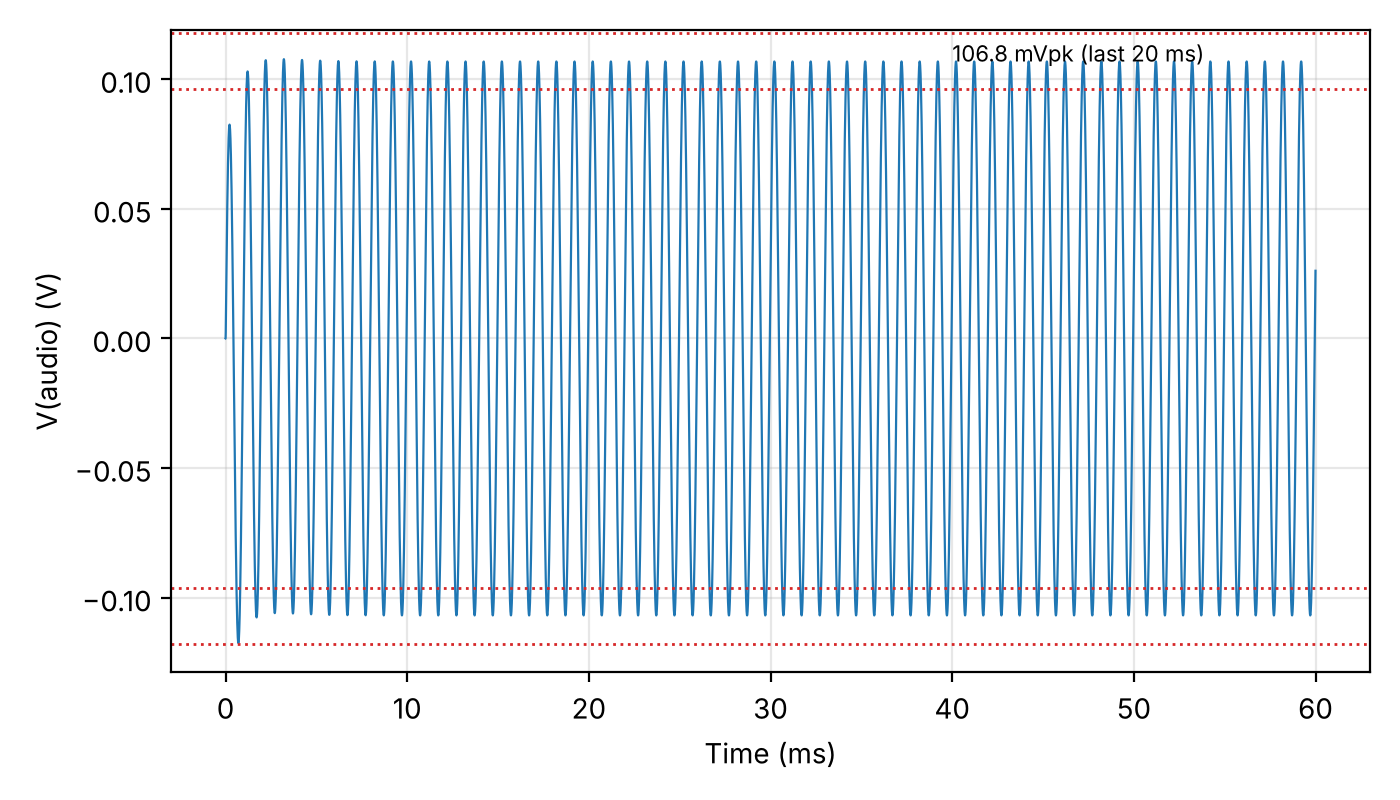
\includegraphics[width=0.5\linewidth]{01b_powerup}
  \caption{Card 1, first power-up configuration (R4 4.7\,k\si{\ohm}, R7 shorted, 10\,mVpk in):
  output peak 106.8\,mVpk against 107\,mVpk expected.}
\end{figure}

\FloatBarrier
\subsection{Cards 2--4: supply and reference}
The supply filter delivers 11.62\,V to the analogue rail. The 3.2\,mVpp on the rail is mostly the
filter still settling; the 150\,kHz switching ripple itself is under 0.2\,mVpp. The the half-rail reference rejects that ripple by more than 160\,dB. With the supply reversed,
the protection diode holds the rail at $-11$\,mV.

\begin{figure}[htbp]
  \centering
  \begin{subfigure}{0.49\linewidth}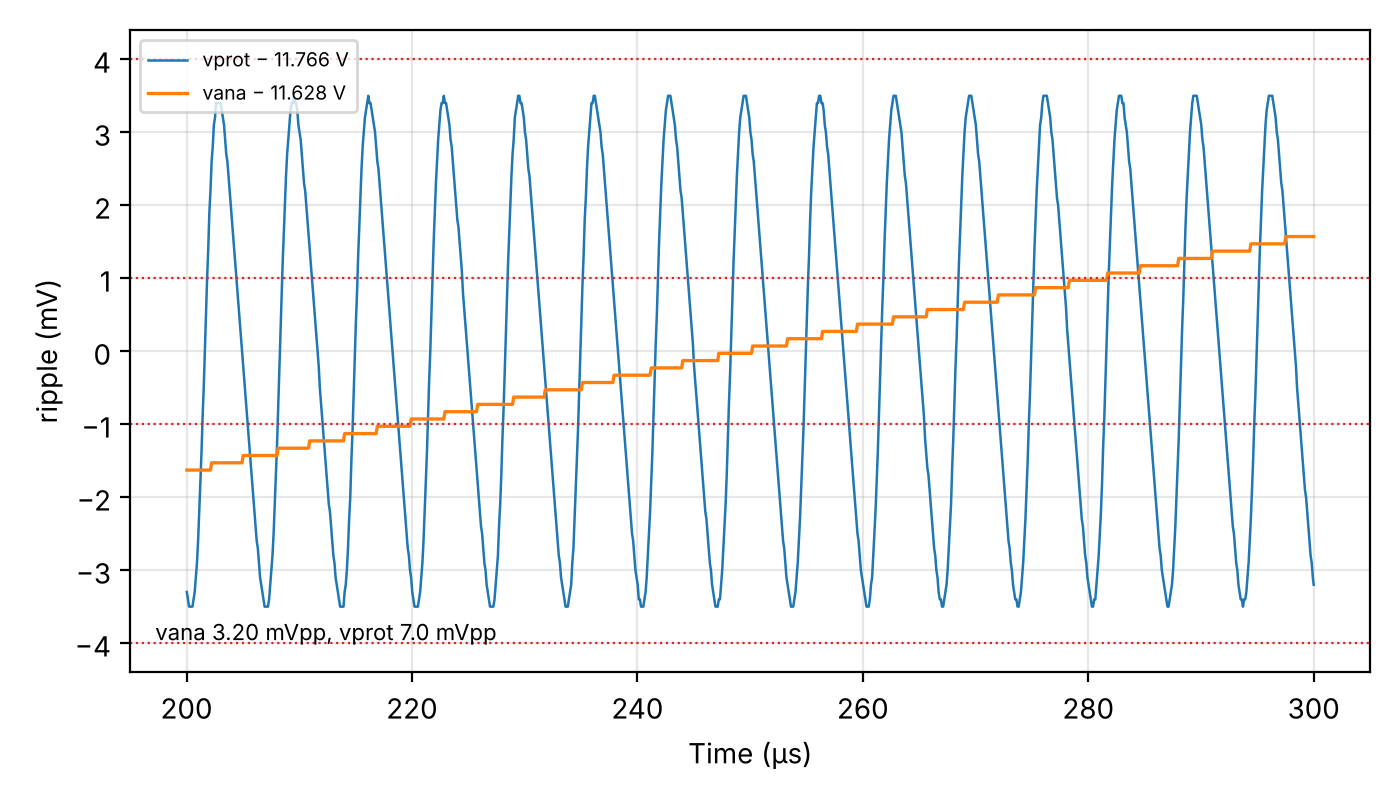
\includegraphics[width=\linewidth]{03_ripple}\caption{Ripple on vana}\end{subfigure}
  \begin{subfigure}{0.49\linewidth}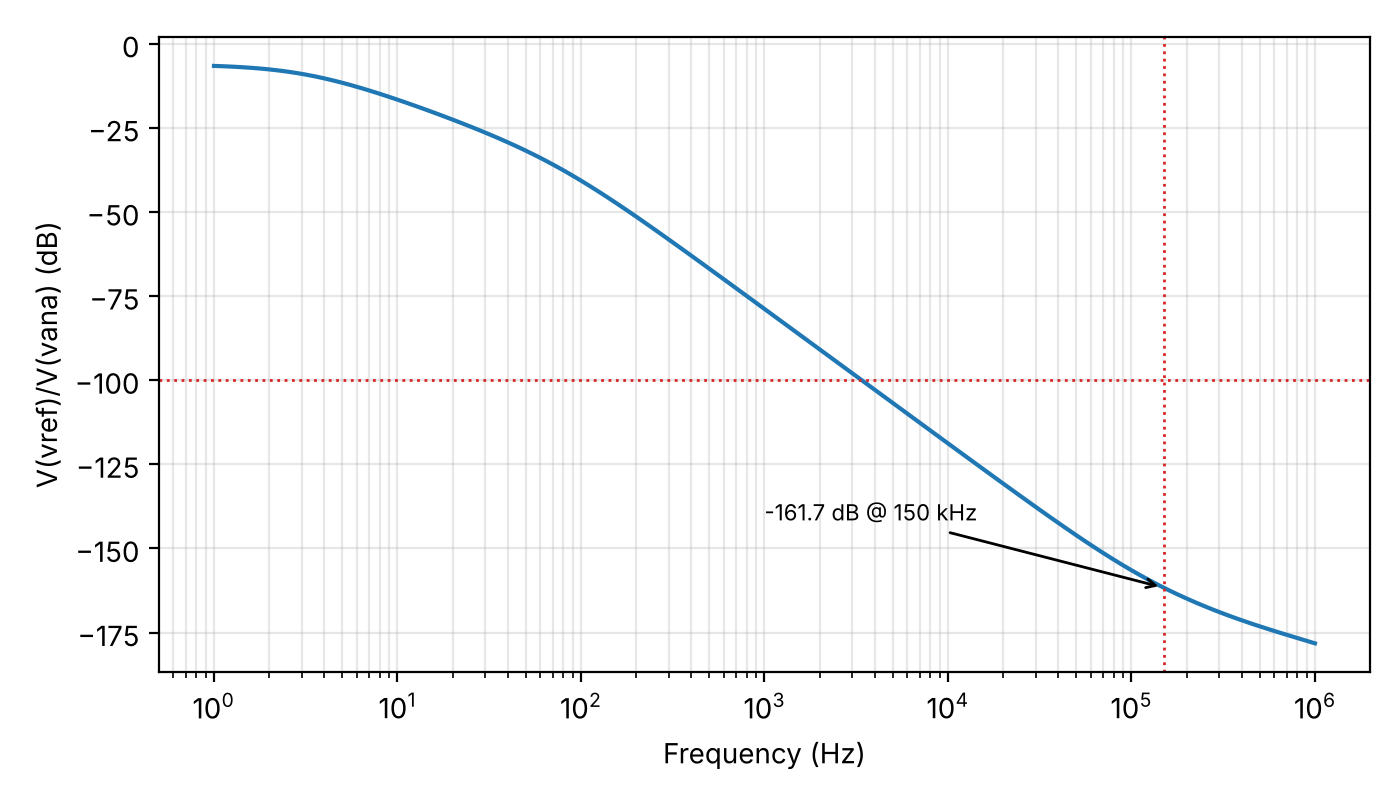
\includegraphics[width=\linewidth]{02_rejection}\caption{Ripple rejection to vref}\end{subfigure}
  \caption{Cards 3 and 2.}
\end{figure}

\FloatBarrier
\subsection{Cards 5--6: sync divider and IF input}
\begin{figure}[htbp]
  \centering
  \begin{subfigure}{0.49\linewidth}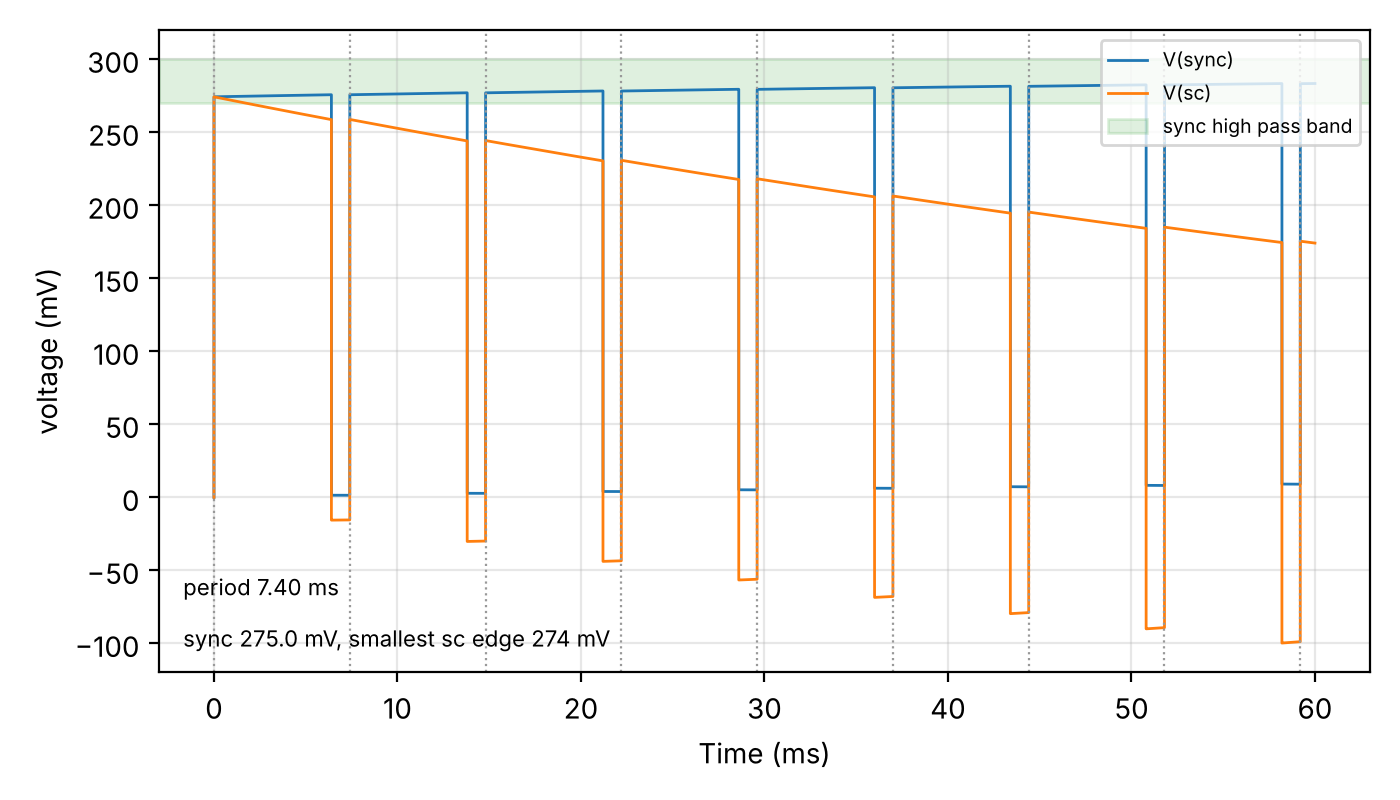
\includegraphics[width=\linewidth]{05_sync_sc}\caption{Sync divider}\end{subfigure}
  \begin{subfigure}{0.49\linewidth}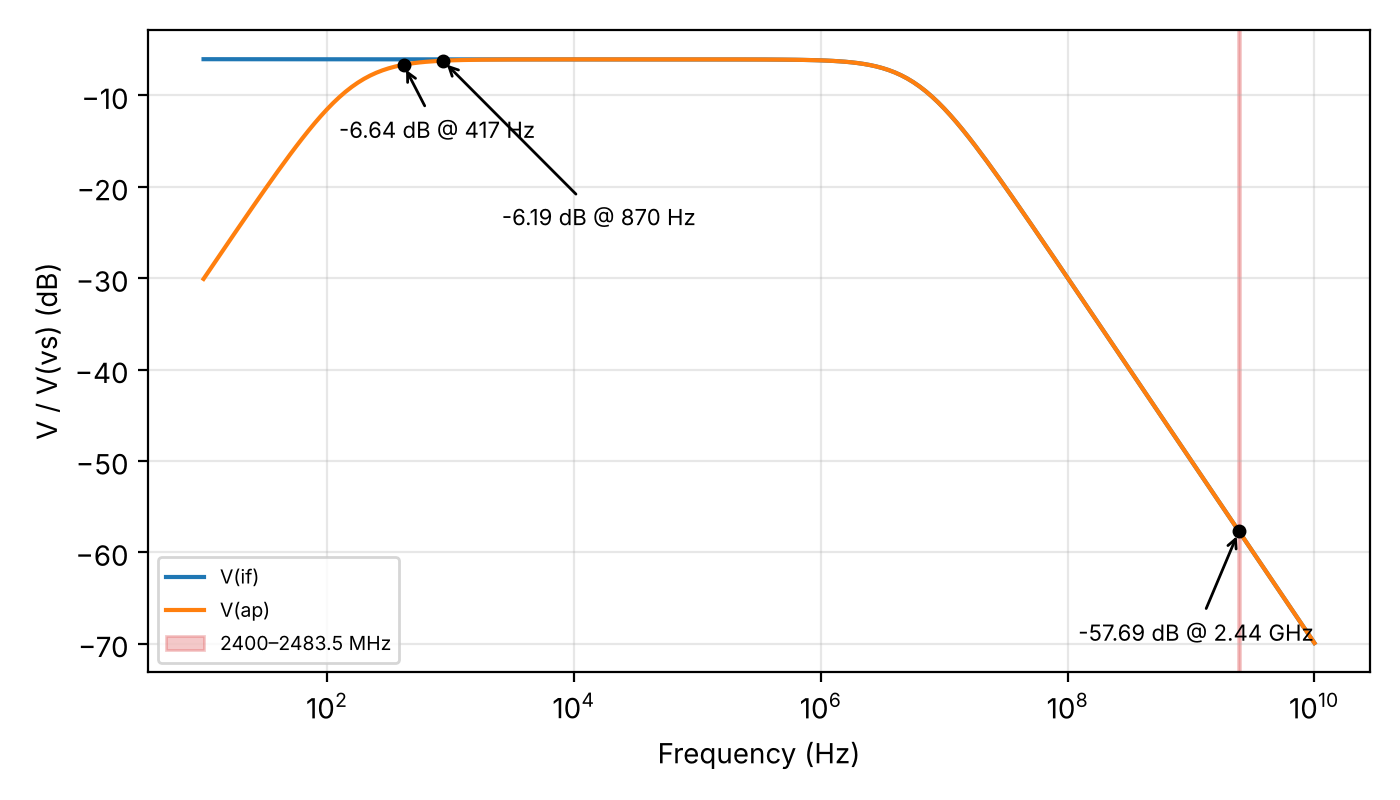
\includegraphics[width=\linewidth]{06_if_input}\caption{IF input network}\end{subfigure}
  \caption{(a) Card 5: the 3.3\,V sync pulse divided down to 275\,mV. (b) Card 6: the
  input network passes the beat frequencies ($-6$\,dB) and blocks 2.44\,GHz ($-58$\,dB).}
\end{figure}

\FloatBarrier
\subsection{Card 7: the radar, scaled}
A scaled model of the full radar (ramp, VCO, delay lines for the target, mixer and IF filter) checks
that a target at range $R$ produces a beat at $f_b = 2BR/(cT)$. The simulated beat frequency is
within 0.05\% of the formula at 5, 10 and 15\,m (Figure~\ref{fig:radar}).

\begin{figure}[htbp]
  \centering
  \begin{subfigure}{0.49\linewidth}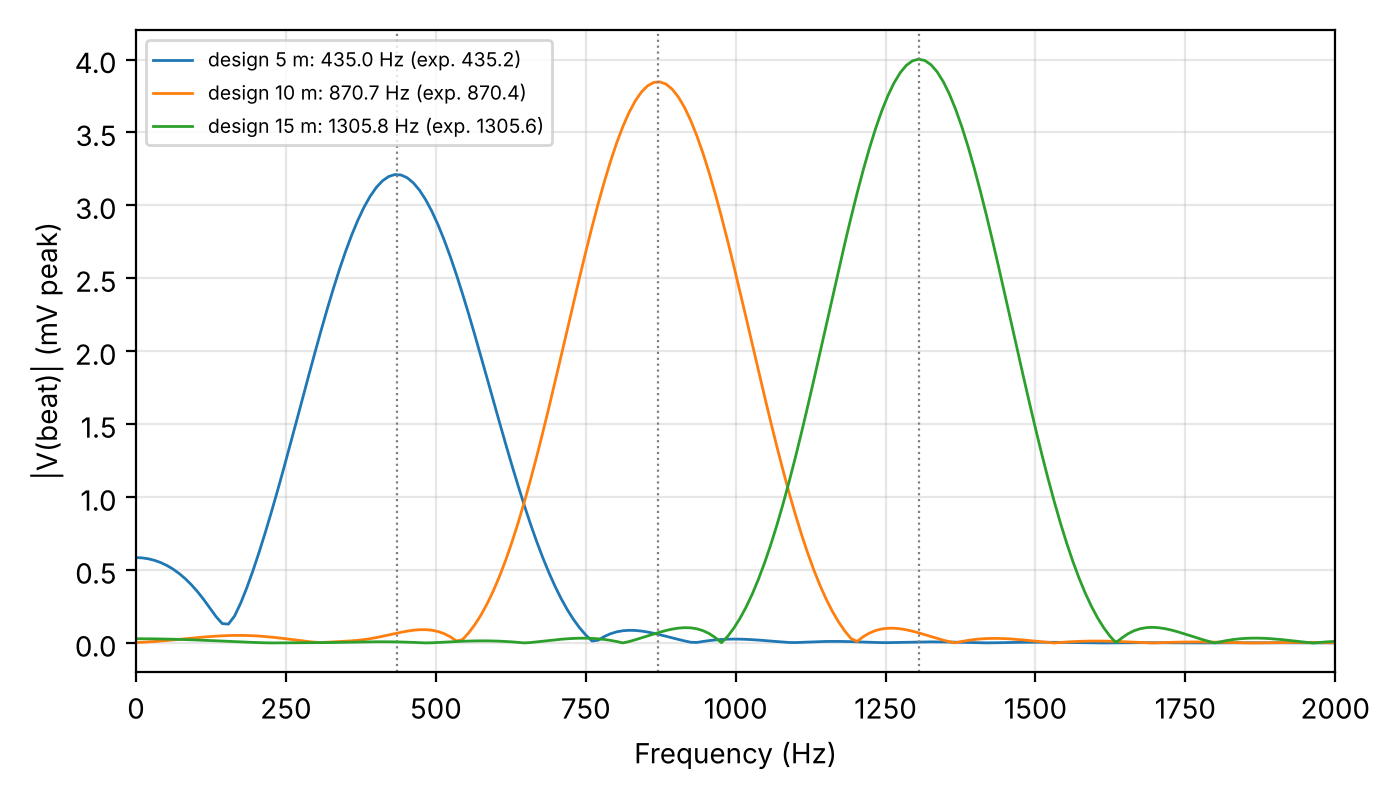
\includegraphics[width=\linewidth]{07_spectra_by_range}\caption{Beat spectra}\end{subfigure}
  \begin{subfigure}{0.49\linewidth}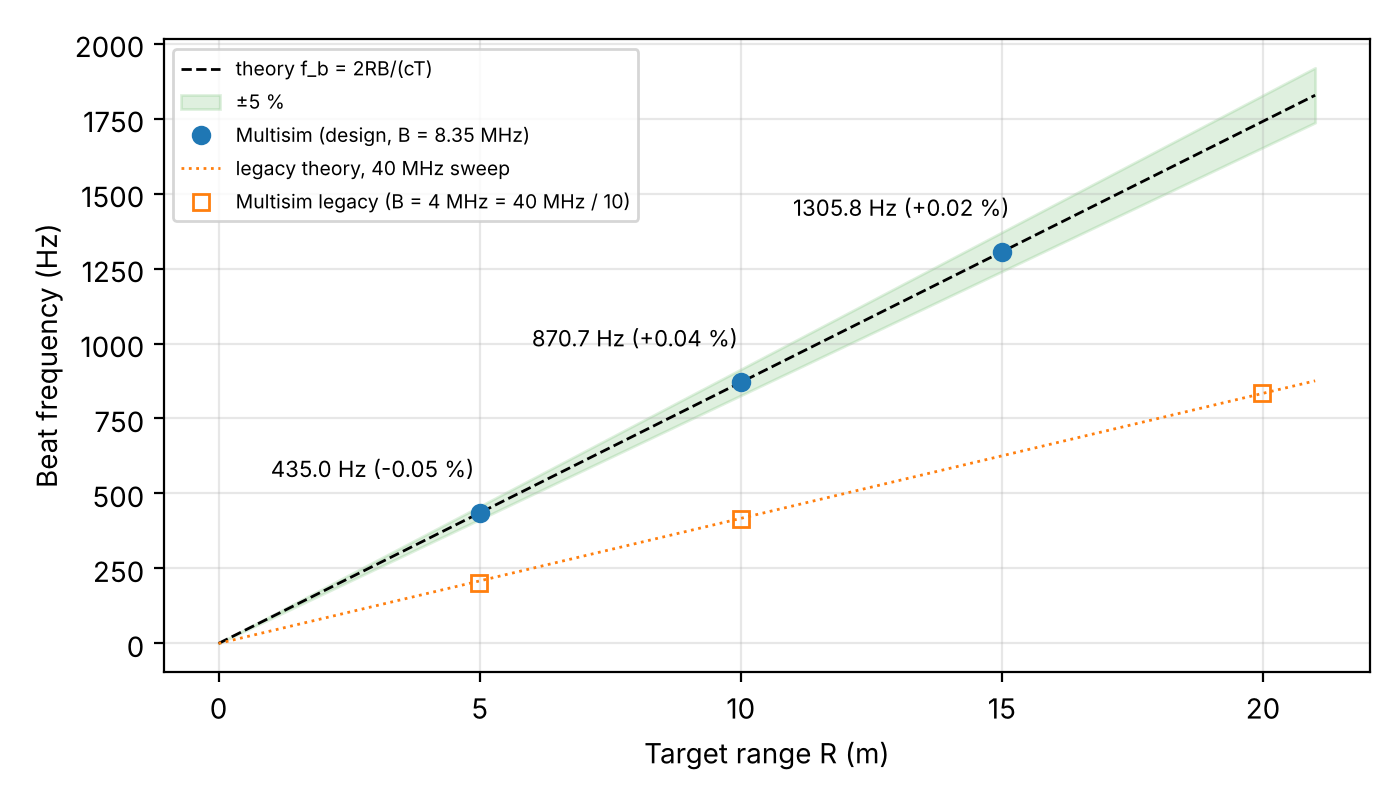
\includegraphics[width=\linewidth]{07_beat_vs_range}\caption{Beat vs.\ range}\end{subfigure}
  \caption{Card 7. (a) Beat spectra for targets at 5, 10 and 15\,m; dotted lines are $2BR/(cT)$.
  (b) Simulated beat frequency against the formula.}
  \label{fig:radar}
\end{figure}

\FloatBarrier
\subsection{Card 8: full board}\label{sec:card8}
\textbf{First result.} With cards 1, 2, 3 and 5 on one sheet, the amplifier's DC point came out latched:
first op-amp at the top rail, second near ground (outputs up to 4.4\,V off vref).

\textbf{Cause.} The netlist Multisim exports for the sheet showed U1A's negative supply pin and U1B's
positive supply pin unconnected. The two halves of U1 had each lost one supply wire when the cards were
pasted together. With no negative supply, U1A's input stage had nowhere to send its bias current except out
of the input pins, which is the 120\,\si{\micro\ampere} seen at its input. Connecting both pins puts every
amplifier output at vref.

\textbf{Design problem found next.} With the wiring fixed, the amplifier now runs off the real reference
(buffer, 47\,\si{\ohm}, 47\,\si{\micro\farad}) instead of an ideal 5.7\,V source. Its gain was then up to 6.4\,dB
low around 200\,Hz (Figure~\ref{fig:c8ac}). Signal currents from the second stage flow into vref and move it
slightly. The first stage's gain resistor (R4, 1\,k\si{\ohm}) returns to vref, so it amplifies that movement by
100 and cancels part of the wanted signal. Raising C6 to 3.3\,mF holds vref still at audio frequencies, and
card 8 then matches card 1 to within 0.15\,dB. Nothing else changes; card 2's DC levels stay the same and its
ripple rejection improves.

\begin{figure}[htbp]
  \centering
  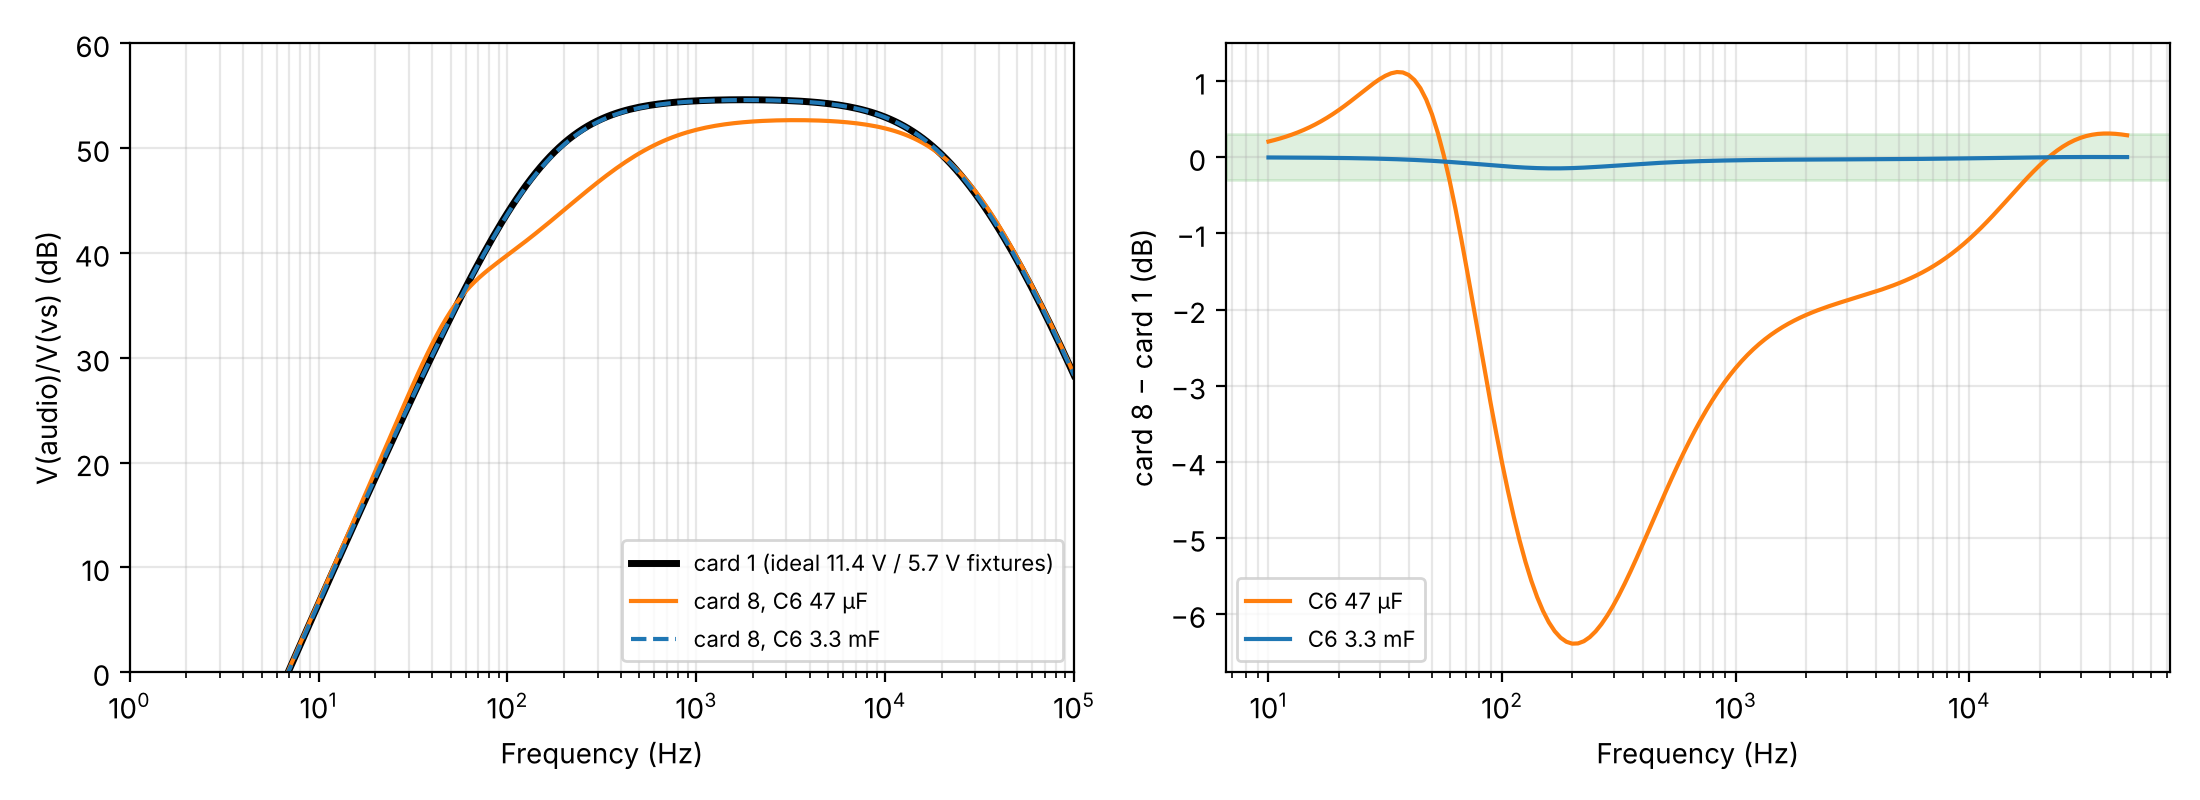
\includegraphics[width=\linewidth]{08_ac_vs_card1}
  \caption{Card 8 gain against card 1. Left: full response. Right: difference; the shaded band is
  the $\pm0.3$\,dB requirement.}
  \label{fig:c8ac}
\end{figure}

\textbf{Power-up.} The op-amp model cannot be solved below about 4.4\,V of supply, so the start-up run
steps the 12\,V input from 6\,V. All three amplifier outputs follow vref up and settle within 0.53\,s with
no latch-up (Figure~\ref{fig:c8pu}). The larger C6 makes vref take about 0.6\,s to settle. Still worth checking on
the bench: power-cycle the board a few times and confirm aout, bout and obuf settle at vref.

\begin{figure}[htbp]
  \centering
  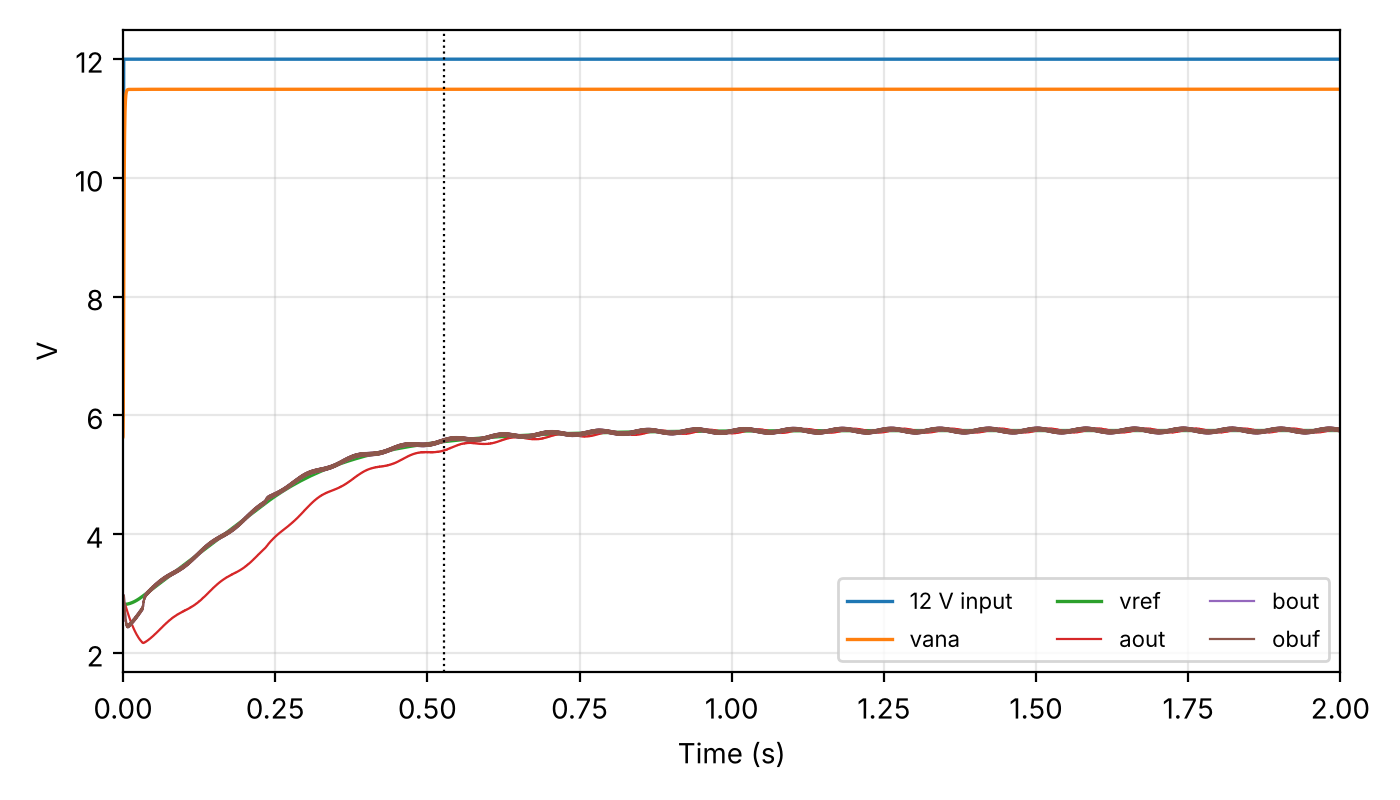
\includegraphics[width=0.6\linewidth]{08_powerup}
  \caption{Card 8 start-up with the corrected sheet. The small wobble after 0.6\,s is the 12.5\,Hz test tone.}
  \label{fig:c8pu}
\end{figure}

All card 8 results above are Multisim runs of the corrected project, exported from Multisim's grapher and
evaluated with a Python script; the 47\,\si{\micro\farad} curve in
Figure~\ref{fig:c8ac} is the same sheet with C6 set back temporarily. Two Multisim details:
\begin{itemize}
  \item Multisim limits the time step to 1/32 of the period of the fastest source on the sheet, even a source set
        to 0\,V. With the 150\,kHz ripple source present, the 1.2\,s two-tone run took 0.2\,\si{\micro\second} steps
        and stopped at 0.126\,s. For the two-tone and power-up runs the ripple source was set to 0\,V and 1\,Hz;
        the ripple check is its own 2\,ms run.
  \item The power-up run also needs a small convergence aid in the op-amp model (1\,pF and 10\,\si{\ohm} on its
        input transistors); with the stock model it stops after 22\,ms. All other runs use the stock model, and
        the saved project keeps it.
\end{itemize}
The same checks repeated in ngspice on Multisim's exported netlist give the same numbers. The supply rail reads 11.49\,V rather than 11.5--11.7\,V only
because the TI model draws 5.7\,mA per op-amp; the TL072 datasheet maximum is 2.5\,mA, which gives 11.62\,V.

\end{document}
